\chapter{How to create a new performance tableau instance}
\label{sec:4}

\abstract*{To be written.}

\abstract{To be written.}

In this tutorial we illustrate a way of creating a new {\em PerformanceTableau\/} instance by editing a template with 5 decision alternatives, 3 decision objectives and 6 performance criteria. 

\section{Editing a template file}
\label{sec:4.1}

For this purpose we provide the following {\tt perfTab\_Template.py} file in the \texttt{examples} directory of the \Digraph resources.

\begin{lstlisting}[caption={PerformanceTableau object template},label=list:4.1,basicstyle=\footnotesize]
   ###############################################
   # Digraph3 documentation
   # Template for creating a new PerformanceTableau instance
   # (C) R. Bisdorff Mar 2021
   # Digraph3/examples/perfTab_Template.py
   ###############################################
   from decimal import Decimal
   from collections import OrderedDict
   #####
   # edit the decision actions
   # avoid special characters, like '_', '/' or ':',
   # in action identifiers and short names
   actions = OrderedDict([
    ('a1', {
     'shortName': 'action1',
     'name': 'decision alternative a1',
     'comment': 'some specific features of this alternative',
      }),
     ...
     ...
   ])
   #####
   # edit the decision objectives
   # adjust the list of performance criteria
   # and the total weight (sum of the criteria weights)
   # per objective
   objectives = OrderedDict([
    ('obj1', {
     'name': 'decision objective obj1',
     'comment': "some specific features of this objective",
     'criteria': ['g1', 'g2'],
     'weight': Decimal('6'),
     }),
     ...
     ...
    ])
   #####
   # edit the performance criteria
   # adjust the objective reference
   # Left Decimal of a threshold = constant part and
   #  right Decimal = proportional part of the threshold 
   criteria = OrderedDict([
    ('g1', {
     'shortName': 'crit1',
     'name': "performance criteria 1",
     'objective': 'obj1',
     'preferenceDirection': 'max',
     'comment': 'measurement scale type and unit',
     'scale': (Decimal('0.0'), Decimal('100.0'),
     'thresholds': {'ind':  (Decimal('2.50'), Decimal('0.0')),
		    'pref': (Decimal('5.00'), Decimal('0.0')),
		    'veto': (Decimal('60.00'), Decimal('0.0'))
                   },
     'weight': Decimal('3'),
     }),
     ...
     ...
    ])
   #####
   # default missing data symbol = -999
   NA = Decimal('-999')
   #####
   # edit the performance evaluations
   # criteria to be minimized take negative grades
   evaluation = {
    'g1': {
       'a1':Decimal("41.0"),
       'a2':Decimal("100.0"),
       'a3':Decimal("63.0"),
       'a4':Decimal('23.0'),
       'a5': NA,
      },
    # g2 is of ordinal type and scale 0-10
    'g2': {
       'a1':Decimal("4"),
       'a2':Decimal("10"),
       'a3':Decimal("6"),
       'a4':Decimal('2'),
       'a5':Decimal('9'),
      },
    # g3 has preferenceDirection = 'min'
    'g3': {
       'a1':Decimal("-52.2"),
       'a2':NA,
       'a3':Decimal("-47.3"),
       'a4':Decimal('-35.7'),
       'a5':Decimal('-68.00'),
      },
    ...
    ...
    }
   ####################
\end{lstlisting}
The template file, shown in Listing \ref{list:4.1}, contains first the instructions to import the required {\tt Decimal} and {\tt OrderedDict} classes (see Lines 7-8). Four main sections are following: the potential decision \emph{actions}, the decision \emph{objectives}, the performance \emph{criteria}, and finally the performance \emph{evaluation}.  

\section{Editing the decision alternatives}
\label{sec:4.2}

Decision alternatives are stored in attribute \texttt{actions} under the \texttt{OrderedDict} format. The \texttt{OrderedDict} object keeps this given order when iterating over the decision alternatives \footnote{See the \href{https://docs.python.org/3/library/collections.html}{{\tt OrderedDict}} description in the Python documentation \citep{python}.}.

Required attributes of each decision alternative, besides the object identifier\footnote{Mind that \emph{graphviz} drawings require node identifier strings without any special characters like `\_` or `/`.},  are: \texttt{shortName}, \texttt{name} and \texttt{comment} (see Lines 15-17). The \texttt{shortName} attribute is essentially used when showing the performance tableau or the performance heatmap in a browser view.


The random performance tableau models, introduced in Chapter \ref{sec:5}, use the \texttt{actions} attribute for storing special features of the decision alternatives. The \emph{Cost-Benefit} model, for instance, uses a \texttt{type} attribute for distinguishing between \emph{advantageous}, \emph{neutral} and \emph{cheap} alternatives (see Section \ref{sec:5.3}). The \emph{3-Objectives} model keeps a detailed record of the performance profile per decision objective and the corresponding random generators per performance criteria (see Lines 7- below).
\begin{lstlisting}
>>> t = Random3ObjectivesPerformanceTableau()
>>> t.actions
    OrderedDict([
     ('p01', {'shortName': 'p01',
              'name': 'action p01 Eco~ Soc- Env+',
              'comment': 'random public policy',
	      'Eco': 'fair',
	      'Soc': 'weak',
	      'Env': 'good',
              'profile': {'Eco':'fair',
	                  'Soc':'weak',
			  'Env':'good'}
              'generators': {'ec01': ('triangular', 50.0, 0.5),
                             'so02': ('triangular', 30.0, 0.5),
		             'en03': ('triangular', 70.0, 0.5),
		             ...
		             },
              }
         ),
      ...
      ])
\end{lstlisting}

The second section of the template file concerns the decision \emph{objectives}.

\section{Editing the decision objectives}
\label{sec:4.3}

The minimal required attributes (see Listing \ref{list:4.1} Lines 27-33) of the ordered decision \textbf{objectives} dictionary, besides the individual objective identifiers, are \texttt{name}, \texttt{comment}, \texttt{criteria} (the list of significant performance criteria) and \texttt{weight} (the importance of the decision objective). The latter attribute contains the sum of the \emph{significance} weights of the objective's criteria list. 

The \texttt{objectives} attribute is methodologically useful for specifying the performance criteria significance in building decision recommendations. Mostly, we assume indeed that decision objectives are all equally important and the performance criteria are equi-significant per objective. This is, for instance, the default setting in the random \emph{3-Objectives} performance tableau model.

\begin{lstlisting}[caption={Example of decision objectives' description},label=list:4.2,basicstyle=\footnotesize]
>>> t = Random3ObjectivesPerformanceTableau()
>>> t.objectives
 OrderedDict([
 ('Eco',
  {'name': 'Economical aspect',
   'comment': 'Random3ObjectivesPerformanceTableau generated',
   'criteria': ['ec01', 'ec06', 'ec09'],
   'weight': Decimal('48')}),
  ('Soc',
   {'name': 'Societal aspect',
    'comment': 'Random3ObjectivesPerformanceTableau generated',
    'criteria': ['so02', 'so12'],
    'weight': Decimal('48')}),
  ('Env',
   {'name': 'Environmental aspect',
    'comment': 'Random3ObjectivesPerformanceTableau generated',
    'criteria': ['en03', 'en04', 'en05', 'en07',
                 'en08', 'en10', 'en11', 'en13'],
    'weight': Decimal('48')})
 ])
\end{lstlisting}

The importance weight sums up to 48 for each one of the three example decision objectives shown in Listing \ref{list:4.2} (Lines 8,13 and 19), so that the significance of each one of the 3 economic criteria is set to 16, of both societal criteria is set to 24, and of each one of the 6 environmental criteria is set to 8.

Mind that the \texttt{objectives} attribute is always present in a \texttt{PerformanceTableau} object instance, even when empty. In this case, we consider that each performance criterion canonically represents in fact its own decision objective. The criterion significance equals in this case the corresponding decision objective's importance weight.

The third section of the template file concerns now the \textbf{performance criteria}.

\section{Editing the family of performance criteria}
\label{sec:4.4}

In order to assess how well each potential decision alternative is satisfying a given decision objective, we need \emph{performance criteria}, i.e. decimal-valued grading functions gathered in an ordered \texttt{criteria} dictionary. The required attributes (see Listing \ref{list:4.3}), besides the criteria identifiers, are the usual \texttt{shortName}, \texttt{name} and \texttt{comment}. Specific for a criterion are furthermore the \texttt{objective} reference, the significance \texttt{weight}, the grading \texttt{scale} (minimum and  maximum performance values), the \texttt{preferenceDirection} ('max' or 'min') and the performance discrimination \texttt{thresholds} attributes.

\begin{lstlisting}[caption={Example of performance criteria description},label=list:4.3,basicstyle=\footnotesize]
   criteria = OrderedDict([
    ('g1', {
     'shortName': 'crit1',
     'name': "performance criteria 1",
     'comment': 'measurement scale type and unit',
     'objective': 'obj1',
     'weight': Decimal('3'),
     'scale': (Decimal('0.0'), Decimal('100.0'),
     'preferenceDirection': 'max',
     'thresholds': {'ind':  (Decimal('2.50'), Decimal('0.0')),
		    'pref': (Decimal('5.00'), Decimal('0.0')),
		    'veto': (Decimal('60.00'), Decimal('0.0'))
                   },
     }),
    ...
    ...])
\end{lstlisting}

In our bipolar-valued outranking approach, all performance criteria implement \emph{decimal-valued} grading functions, where preferences are either \emph{increasing} or \emph{decreasing} with measured performances.

In order to model a \textbf{coherent} performance tableau, the decision criteria must satisfy two methodological requirements:
\begin{enumerate}
\item \textbf{Independance}: Each decision criterion implements a grading that is \emph{functionally independent} of the grading of the other decision criteria, i.e. the performance measured on one of the criteria does not \emph{constrain} in any sense the performance measured on any other criterion.
\item \textbf{Non redundancy}: Each performance criterion is only \emph{significant} for a \emph{single} decision objective.
\end{enumerate}

In order to take into account any, usually \emph{unavoidable}, \textbf{imprecision} of the performance grading procedures, we may specify three performance \textbf{discrimination thresholds}: an \emph{indifference} ('ind'), a \emph{preference} ('pref') and a \emph{considerable performance difference} ('veto') threshold (see Listing \ref{list:4.3} Lines 10-12). The left decimal number of a threshold description tuple indicates a \emph{constant part}, whereas the right decimal number indicates a \emph{proportional} part.

On the template performance criterion $g_1$, shown in Listing \ref{list:4.3}, we observe for instance a grading scale from $0.0$ to $100.0$ with a constant \emph{indifference} threshold of $2.5$, a constant \emph{preference} threshold of $5.0$, and a constant \emph{considerable performance difference} threshold of $60.0$. The latter threshold  will trigger, the case given, a \emph{polarisation} of the outranking statement \citep{BIS-2013}.

In a random \emph{Cost-Benefit} performance tableau model we may obtain by default the following content.

\begin{lstlisting}[caption={Example of cardinal Costs criterion},label=list:4.4,basicstyle=\footnotesize]
>>> tcb = RandomCBPerformanceTableau()
>>> tcb.showObjectives()
 *------ decision objectives -------*
 C: Costs
   c1 random cardinal cost criterion 6
   Total weight: 6.00 (1 criteria)
   ...
   ...
>>> tcb.criteria
 OrderedDict([
  ('c1', {'preferenceDirection': 'min',
          'scaleType': 'cardinal',
	  'objective': 'C',
	  'shortName': 'c1',
	  'name': 'random cardinal cost criterion',
	  'scale': (0.0, 100.0),
	  'weight': Decimal('6'),
	  'randomMode': ['triangular', 50.0, 0.5],
	  'comment': 'Evaluation generator: triangular law ...',
          'thresholds': OrderedDict([
	     ('ind', (Decimal('1.49'), Decimal('0'))),
	     ('pref', (Decimal('3.7'), Decimal('0'))),
	     ('veto', (Decimal('67.71'), Decimal('0')))
             ])
           }),
  ...
  ...
 ])
\end{lstlisting}

Criterion $c1$ appears here (see Listing \ref{list:4.4}) to be a cardinal criterion to be minimized and significant for the \emph{Costs} ($C$) decision objective. We may use the {\tt showCriteria()} method for printing the corresponding performance discrimination thresholds.

\begin{lstlisting}[basicstyle=\footnotesize]
>>> tcb.showCriteria(IntegerWeights=True)
 *----  criteria -----*
  c1 'Costs/random cardinal cost criterion'
    Scale = (0.0, 100.0)
    Weight = 6 
    Threshold ind : 1.49 + 0.00x ; percentile: 5.13
    Threshold pref : 3.70 + 0.00x ; percentile: 10.26
    Threshold veto : 67.71 + 0.00x ; percentile: 96.15
\end{lstlisting}

The \emph{indifference} threshold on this criterion amounts to a constant value of $1.49$ (Line 6 above). More or less $5\%$ of the observed performance differences on this criterion appear hence to be \textbf{insignificant}. Similarly, with a preference threshold of $3.70$, about $90\%$ of the observed performance differences are preferentially \textbf{significant} (Line 7). Furthermore, $100.0 - 96.15 = 3.85\%$ of the observed performance differences appear to be \textbf{considerable} (Line 8) and will trigger a \emph{polarisation} of the corresponding outranking statements.

After the performance criteria description, we are ready for recording the actual \textbf{performance table}.

\section{Editing the performance table}
\label{sec:4.5}

The individual grades of each decision alternative on each decision criterion are recorded in a double \emph{criterion} x \emph{action} dictionary called \texttt{evaluation} (see Listing \ref{list:4.4}). As we may encounter missing data cases, we previously define a \emph{missing data} symbol \texttt{NA} which is set here to a value disjoint from all the measurement scales, by default \texttt{Decimal('-999')} (Line 2).

\begin{lstlisting}[caption={Editing performance grades},label=list:4.5,basicstyle=\footnotesize]
#----------
NA = Decimal('-999')
#----------
evaluation = {
  'g1': {
     'a1':Decimal("41.0"),
     'a2':Decimal("100.0"),
     'a3':Decimal("63.0"),
     'a4':Decimal('23.0'),
     'a5': NA,  # missing data
   },
   ...
   ...
  # g3 has preferenceDirection = 'min'
  'g3': {
     'a1':Decimal("-52.2"), # negative grades
     'a2':NA,
     'a3':Decimal("-47.3"),
     'a4':Decimal('-35.7'),
     'a5':Decimal('-68.00'),
   },
   ...
   ...
}
\end{lstlisting}

Notice in Listing \ref{list:4.4} (Lines 16- ) that on a criterion with \texttt{preferenceDirection} = 'min' all performance grades are recorded as \textbf{negative} values.

We may now inspect the eventually recorded complete template performance table.

\begin{lstlisting}[basicstyle=\footnotesize]
>>> from perfTabs import PerformanceTableau   
>>> t = PerformanceTableau('perfTab_Template')
>>> t.showPerformanceTableau(ndigits=1)
 *----  performance tableau -----*
  Criteria  |  'g1'   'g2'  'g3'  'g4'   'g5'   'g6'   
  Actions   |    3      3     6     2      2      2    
   ---------|-----------------------------------------
  'action1' |  41.0   4.0  -52.2  71.0   63.0   22.5  
  'action2' | 100.0  10.0    NA   89.0   30.7   75.0  
  'action3' |  63.0   6.0  -47.3  55.4   63.5    NA   
  'action4' |  23.0   2.0  -35.7  83.5   37.5   54.9  
  'action5' |   NA    9.0  -68.0  10.0   88.0   75.0
\end{lstlisting}

We may furthermore compute the associated outranking digraph and check if we observe any polarised outranking situtations.

\begin{lstlisting}[basicstyle=\footnotesize]
>>> from outrankingDigraphs import BipolarOutrankingDigraph
>>> g = BipolarOutrankingDigraph(t)
>>> g.showVetos()
 *----  Veto situations ---
  number of veto situations : 1 
  1: r(a4 >= a2) = -0.44
     criterion: g1
     Considerable performance difference : -77.00
     Veto discrimination threshold       : -60.00
     Polarisation: r(a4 >= a2) = -0.44 ==> -1.00
 *----  Counter-veto situations ---
  number of counter-veto situations : 1 
  1: r(a2 >= a4) = 0.56
     criterion: g1
     Considerable performance difference : 77.00
     Counter-veto threshold              : 60.00
     Polarisation: r(a2 >= a4) = 0.56 ==> +1.00
\end{lstlisting}

Indeed, due to the considerable performance difference ($77.00$) oberved on performance criterion $g1$, alternative $a2$ \textbf{for sure} \emph{outranks} alternative $a4$, respectively $a4$ \textbf{for sure} \emph{does not outrank} $a2$.

\section{Inspecting the template outranking relation}
\label{sec:4.6}

Let us have a look at the outranking relation table.

\begin{lstlisting}[caption={The template outranking relation},label=list:4.5,basicstyle=\footnotesize]
>>> g.showRelationTable()
 * ---- Relation Table -----
   r   |  'a1'   'a2'   'a3'   'a4'   'a5'   
  -----|-----------------------------------
  'a1' | +1.00  -0.44  -0.22  -0.11  +0.06  
  'a2' | +0.44  +1.00  +0.33  +1.00  +0.28  
  'a3' | +0.67  -0.33  +1.00  +0.00  +0.17  
  'a4' | +0.11  -1.00  +0.00  +1.00  +0.06  
   'a5' | -0.06  -0.06  -0.17  -0.06  +1.00
\end{lstlisting}

We may notice in the outranking relation table above (see Listing \ref{list:4.5}) that decision alternative $a2$ positively \textbf{outranks} all the other four alternatives  (Line 6). Similarly, alternative $a5$ is positively \textbf{outranked} by all the other alternatives (see Line 9). We may orient this way the \emph{graphviz} drawing of the template outranking digraph. 

\begin{lstlisting}[basicstyle=\footnotesize]
>>> g.exportGraphViz(fileName= 'template',\
...                  bestChoice =['a2'],\
...                  worstChoice=['a5'])
  *---- exporting a dot file for GraphViz tools ---------*
   Exporting to template.dot
   dot -Grankdir=BT -Tpng template.dot -o template.png
\end{lstlisting}
    
\begin{figure}[h]
\sidecaption
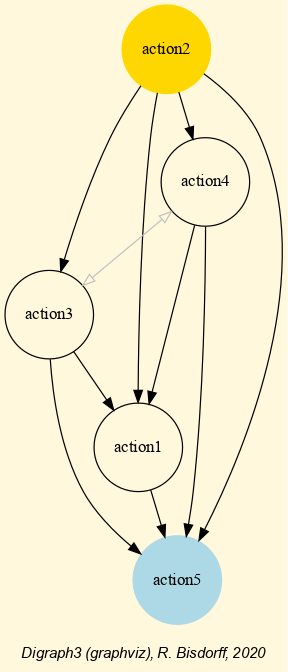
\includegraphics[width=4cm]{Figures/template.png}
\caption{The template outranking digraph models in fact a \textbf{partial order} on the five potential decision alternatives. Alternatives \emph{action3} ($a3$ ) and \emph{action4} ($a4$) appear actually \textbf{incomparable}.}
\label{fig:4.1}       % Give a unique label
\end{figure}

In Listing \ref{list:4.5} their pairwise outranking characteritics show indeed the \textbf{indeterminate} value $0.00$ (Lines 7-8). We may check their pairwise comparison as follows.

\begin{lstlisting}[basicstyle=\footnotesize]
>>> g.showPairwiseComparison('a3','a4')
 *------------  pairwise comparison ----*
  Comparing actions : ('a3','a4')
  crit. wght.  g(x)   g(y)   diff   | ind   pref   r()  | 
   --------------------------------   -----------------
  'g1' 3.00  63.00   23.00  +40.00 | 2.50  5.00  +3.00 | 
  'g2' 3.00   6.00    2.00   +4.00 | 0.00  1.00  +3.00 | 
  'g3' 6.00 -47.30  -35.70  -11.60 | 0.00 10.00  -6.00 | 
  'g4' 2.00  55.40   83.50  -28.10 | 2.09  4.18  -2.00 | 
  'g5' 2.00  63.50   37.50  +26.00 | 0.00 10.00  +2.00 | 
  'g6'  NA   54.90
  Outranking characteristic value:   r(a3 >= a4) = +0.00
  Valuation in range: -18.00 to +18.00
\end{lstlisting}

The incomparability situation between $a3$ and $a4$ results here from a perfect balancing of positive (+8) and negative (-8) criteria significances.

\section{Ranking the template peformance tableau}
\label{sec:4.7}

We may eventually rank the five decision alternatives with a heatmap browser view following the \emph{Copeland} ranking rule (see Section \ref{sec:7.2}) which consistently reproduces the partial outranking order shown in Fig. \ref{fig:4.1}. 

\begin{lstlisting}[basicstyle=\footnotesize] 
   >>> g.showHTMLPerformanceHeatmap(ndigits=1,colorLevels=5,\
   ...    Correlations=True,rankingRule='Copeland',\
   ...    pageTitle='Heatmap of the template performance tableau')
\end{lstlisting}

\begin{figure}[h]
%\sidecaption
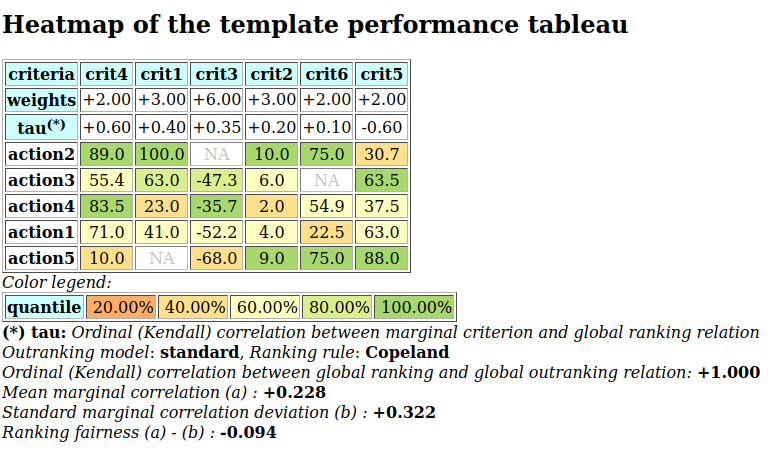
\includegraphics[width=10cm]{Figures/templateHeatmapCop.png}
\caption{Copeland ranked heatmap of the template performance tableau}
\label{fig:4.2}       % Give a unique label
\end{figure}

Due to a 11 against 7 \textbf{plurality tyranny} effect, the \emph{Copeland} ranking rule, essentially based on crisp majority outranking counts, puts here alternative \emph{action5} ($a5$) last, despite its excellent grades observed on criteria $g2$, $g5$ and $g6$. A slightly \textbf{fairer} ranking result may be obtained with the \emph{NetFlows} ranking rule.

\begin{lstlisting}[basicstyle=\footnotesize] 
   >>> g.showHTMLPerformanceHeatmap(ndigits=1,colorLevels=5,\
   ...    Correlations=True,rankingRule='NetFlows',\
   ...    pageTitle='Heatmap of the template performance tableau')
\end{lstlisting}

\begin{figure}[h]
%\sidecaption
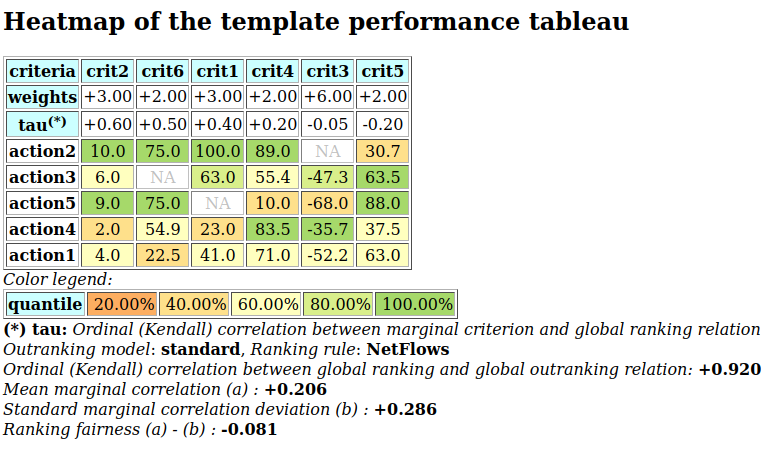
\includegraphics[width=10cm]{Figures/templateHeatmapNF.png}
\caption{Net flows ranked heatmap of the template performance tableau}
\label{fig:4.3}       % Give a unique label
\end{figure}

It might be opportun to furthermore study the robustness of the apparent outranking situations when assuming only *ordinal* or *uncertain* criteria significance weights. If interested in mainly objectively *unopposed* (multipartisan) outranking situations, one might also try the {\tt UnOpposedOutrankingDigraph} constructor. (see Chapter \ref{sec:x}). 
 
%%%%%%% The chapter bibliography
%\normallatexbib
\clearpage
%\phantomsection
%\addcontentsline{toc}{section}{Chapter Bibliography}
\bibliographystyle{spbasic}
\typeout{}
\bibliography{03-backMatters/reference}
%\chapter{How to create a new performance tableau instance}
\label{sec:4}

\abstract*{To be written.}

\abstract{To be written.}

In this tutorial we illustrate a way of creating a new {\em PerformanceTableau\/} instance by editing a template with 5 decision alternatives, 3 decision objectives and 6 performance criteria. 

\section{Editing a template file}
\label{sec:4.1}

For this purpose we provide the following {\tt perfTab\_Template.py} file in the \texttt{examples} directory of the \Digraph resources.

\begin{lstlisting}[caption={PerformanceTableau object template},label=list:4.1,basicstyle=\footnotesize]
   ###############################################
   # Digraph3 documentation
   # Template for creating a new PerformanceTableau instance
   # (C) R. Bisdorff Mar 2021
   # Digraph3/examples/perfTab_Template.py
   ###############################################
   from decimal import Decimal
   from collections import OrderedDict
   #####
   # edit the decision actions
   # avoid special characters, like '_', '/' or ':',
   # in action identifiers and short names
   actions = OrderedDict([
    ('a1', {
     'shortName': 'action1',
     'name': 'decision alternative a1',
     'comment': 'some specific features of this alternative',
      }),
     ...
     ...
   ])
   #####
   # edit the decision objectives
   # adjust the list of performance criteria
   # and the total weight (sum of the criteria weights)
   # per objective
   objectives = OrderedDict([
    ('obj1', {
     'name': 'decision objective obj1',
     'comment': "some specific features of this objective",
     'criteria': ['g1', 'g2'],
     'weight': Decimal('6'),
     }),
     ...
     ...
    ])
   #####
   # edit the performance criteria
   # adjust the objective reference
   # Left Decimal of a threshold = constant part and
   #  right Decimal = proportional part of the threshold 
   criteria = OrderedDict([
    ('g1', {
     'shortName': 'crit1',
     'name': "performance criteria 1",
     'objective': 'obj1',
     'preferenceDirection': 'max',
     'comment': 'measurement scale type and unit',
     'scale': (Decimal('0.0'), Decimal('100.0'),
     'thresholds': {'ind':  (Decimal('2.50'), Decimal('0.0')),
		    'pref': (Decimal('5.00'), Decimal('0.0')),
		    'veto': (Decimal('60.00'), Decimal('0.0'))
                   },
     'weight': Decimal('3'),
     }),
     ...
     ...
    ])
   #####
   # default missing data symbol = -999
   NA = Decimal('-999')
   #####
   # edit the performance evaluations
   # criteria to be minimized take negative grades
   evaluation = {
    'g1': {
       'a1':Decimal("41.0"),
       'a2':Decimal("100.0"),
       'a3':Decimal("63.0"),
       'a4':Decimal('23.0'),
       'a5': NA,
      },
    # g2 is of ordinal type and scale 0-10
    'g2': {
       'a1':Decimal("4"),
       'a2':Decimal("10"),
       'a3':Decimal("6"),
       'a4':Decimal('2'),
       'a5':Decimal('9'),
      },
    # g3 has preferenceDirection = 'min'
    'g3': {
       'a1':Decimal("-52.2"),
       'a2':NA,
       'a3':Decimal("-47.3"),
       'a4':Decimal('-35.7'),
       'a5':Decimal('-68.00'),
      },
    ...
    ...
    }
   ####################
\end{lstlisting}

The template file, shown in Listing \ref{list:4.1}, contains first the instructions to import the required {\tt Decimal} and {\tt OrderedDict} classes (see Lines 7-8). Four main sections are following: the potential decision {\bf actions}, the decision \textbf{objectives}, the performance \textbf{criteria}, and finally the performance \textbf{evaluation}.  

\section{Editing the decision alternatives}
\label{sec:4.2}

Decision alternatives are stored in attribute \textbf{actions} under the \texttt{OrderedDict} format (see the \href{https://docs.python.org/3/library/collections.html}{{\tt OrderedDict}} description in the Python documentation).

Required attributes of each decision alternative, besides the object identifier,  are: \texttt{shortName}, \texttt{name} and \texttt{}comment (see Lines 15-17). The \texttt{shortName} attribute is essentially used when showing the performance tableau or the performance heatmap in a browser view.

\begin{svgraybox}Mind that graphviz drawings require digraph actions' (nodes) identifier strings without any special characters like `\_` or `/`.\end{svgraybox}

Decision actions descriptions are stored in the order of which they appear in the stored instance file. The \texttt{OrderedDict} object keeps this given order when iterating over the decision alternatives.

The random performance tableau models presented in the previous tutorial use the \texttt{actions} attribute for storing special features of the decision alternatives. The \emph{Cost-Benefit} model, for instance, uses a \texttt{type} attribute for distinguishing between \emph{advantageous}, \emph{neutral} and \emph{cheap} alternatives. The \emph{3-Objectives} model keeps a detailed record of the performance profile per decision objective and the corresponding random generators per performance criteria (see Lines 7- below).

\begin{lstlisting}[basicstyle=\footnotesize]
>>> t = Random3ObjectivesPerformanceTableau()
>>> t.actions
    OrderedDict([
     ('p01', {'shortName': 'p01',
              'name': 'action p01 Eco~ Soc- Env+',
              'comment': 'random public policy',
	      'Eco': 'fair',
	      'Soc': 'weak',
	      'Env': 'good',
              'profile': {'Eco':'fair',
	                  'Soc':'weak',
			  'Env':'good'}
              'generators': {'ec01': ('triangular', 50.0, 0.5),
                             'so02': ('triangular', 30.0, 0.5),
		             'en03': ('triangular', 70.0, 0.5),
		             ...
		             },
              }
         ),
      ...
      ])
\end{lstlisting}

The second section of the template file concerns the decision \textbf{objectives}.

\section{Editing the decision objectives}
\label{sec:4.3}

The minimal required attributes (see Listing \ref{list:4.1} Lines 27-33) of the ordered decision \textbf{objectives} dictionary, besides the individual objective identifiers, are \texttt{name}, \texttt{comment}, \texttt{criteria} (the list of significant performance criteria) and \texttt{weight} (the importance of the decision objective). The latter attribute contains the sum of the \emph{significance} weights of the objective's criteria list. 

The \texttt{objectives} attribute is methodologically useful for specifying the performance criteria significance in building decision recommendations. Mostly, we assume indeed that decision objectives are all equally important and the performance criteria are equi-significant per objective. This is, for instance, the default setting in the random \emph{3-Objectives} performance tableau model.

\begin{lstlisting}[caption={Example of decision objectives' description},label=list:4.2,basicstyle=\footnotesize]
>>> t = Random3ObjectivesPerformanceTableau()
>>> t.objectives
 OrderedDict([
 ('Eco',
  {'name': 'Economical aspect',
   'comment': 'Random3ObjectivesPerformanceTableau generated',
   'criteria': ['ec01', 'ec06', 'ec09'],
   'weight': Decimal('48')}),
  ('Soc',
   {'name': 'Societal aspect',
    'comment': 'Random3ObjectivesPerformanceTableau generated',
    'criteria': ['so02', 'so12'],
    'weight': Decimal('48')}),
  ('Env',
   {'name': 'Environmental aspect',
    'comment': 'Random3ObjectivesPerformanceTableau generated',
    'criteria': ['en03', 'en04', 'en05', 'en07',
                 'en08', 'en10', 'en11', 'en13'],
    'weight': Decimal('48')})
 ])
\end{lstlisting}

The importance weight sums up to 48 for each one of the three example decision objectives shown in Listing \ref{list:4.2} (Lines 8,13 and 19), so that the significance of each one of the 3 economic criteria is set to 16, of both societal criteria is set to 24, and of each one of the 6 environmental criteria is set to 8.

\begin{svgraybox}Mind that the \texttt{objectives} attribute is always present in a \texttt{PerformanceTableau} object instance, even when empty. In this case, we consider that each performance criterion canonically represents in fact its own decision objective. The criterion significance equals in this case the corresponding decision objective's importance weight.\end{svgraybox}

The third section of the template file concerns now the \textbf{performance criteria}.

\section{Editing the family of performance criteria}
\label{sec:4.4}

In order to assess how well each potential decision alternative is satisfying a given decision objective, we need \emph{performance criteria}, i.e. decimal-valued grading functions gathered in an ordered \texttt{criteria} dictionary. The required attributes (see Listing \ref{list:4.3}), besides the criteria identifiers, are the usual \texttt{shortName}, \texttt{name} and \texttt{comment}. Specific for a criterion are furthermore the \texttt{objective} reference, the significance \texttt{weight}, the grading \texttt{scale} (minimum and  maximum performance values), the \texttt{preferenceDirection} ('max' or 'min') and the performance discrimination \texttt{thresholds} attributes.

\begin{lstlisting}[caption={Example of performance criteria description},label=list:4.3,basicstyle=\footnotesize]
   criteria = OrderedDict([
    ('g1', {
     'shortName': 'crit1',
     'name': "performance criteria 1",
     'comment': 'measurement scale type and unit',
     'objective': 'obj1',
     'weight': Decimal('3'),
     'scale': (Decimal('0.0'), Decimal('100.0'),
     'preferenceDirection': 'max',
     'thresholds': {'ind':  (Decimal('2.50'), Decimal('0.0')),
		    'pref': (Decimal('5.00'), Decimal('0.0')),
		    'veto': (Decimal('60.00'), Decimal('0.0'))
                   },
     }),
    ...
    ...])
\end{lstlisting}

In our bipolar-valued outranking approach, all performance criteria implement \emph{decimal-valued} grading functions, where preferences are either \emph{increasing} or \emph{decreasing} with measured performances.

\begin{svgraybox}In order to model a \textbf{coherent} performance tableau, the decision criteria must satisfy two methodological requirements:
\begin{enumerate}
\item \textbf{Independance}: Each decision criterion implements a grading that is \emph{functionally independent} of the grading of the other decision criteria, i.e. the performance measured on one of the criteria does not \emph{constrain} the performance measured on any other criterion.
\item \textbf{Non redundancy}: Each performance criterion is only \emph{significant} for a \emph{single} decision objective.
\end{enumerate}
\end{svgraybox}

In order to take into account any, usually \emph{unavoidable}, \textbf{imprecision} of the performance grading procedures, we may specify three performance \textbf{discrimination thresholds}: an \emph{indifference} ('ind'), a \emph{preference} ('pref') and a \emph{considerable performance difference} ('veto') threshold (see Listing \ref{list:4.3} Lines 10-12). The left decimal number of a threshold description tuple indicates a \emph{constant part}, whereas the right decimal number indicates a \emph{proportional} part.

On the template performance criterion $g_1$, shown in Listing \ref{list:4.3}, we observe for instance a grading scale from $0.0$ to $100.0$ with a constant \emph{indifference} threshold of $2.5$, a constant \emph{preference} threshold of $5.0$, and a constant \emph{considerable performance difference} threshold of $60.0$. The latter threshold  will trigger, the case given, a \emph{polarisation} of the outranking statement [BIS-2013].

In a random \emph{Cost-Benefit} performance tableau model we may obtain by default the following content.

\begin{lstlisting}[caption={Example of cardinal Costs criterion},label=list:4.4,basicstyle=\footnotesize]
>>> tcb = RandomCBPerformanceTableau()
>>> tcb.showObjectives()
 *------ decision objectives -------*
 C: Costs
   c1 random cardinal cost criterion 6
   Total weight: 6.00 (1 criteria)
   ...
   ...
>>> tcb.criteria
 OrderedDict([
  ('c1', {'preferenceDirection': 'min',
          'scaleType': 'cardinal',
	  'objective': 'C',
	  'shortName': 'c1',
	  'name': 'random cardinal cost criterion',
	  'scale': (0.0, 100.0),
	  'weight': Decimal('6'),
	  'randomMode': ['triangular', 50.0, 0.5],
	  'comment': 'Evaluation generator: triangular law ...',
          'thresholds': OrderedDict([
	     ('ind', (Decimal('1.49'), Decimal('0'))),
	     ('pref', (Decimal('3.7'), Decimal('0'))),
	     ('veto', (Decimal('67.71'), Decimal('0')))
             ])
           }),
  ...
  ...
 ])
\end{lstlisting}

Criterion $c1$ appears here (see Listing \ref{list:4.4}) to be a cardinal criterion to be minimized and significant for the \emph{Costs} ($C$) decision objective. We may use the {\tt showCriteria()} method for printing the corresponding performance discrimination thresholds.

\begin{lstlisting}[basicstyle=\footnotesize]
>>> tcb.showCriteria(IntegerWeights=True)
 *----  criteria -----*
  c1 'Costs/random cardinal cost criterion'
    Scale = (0.0, 100.0)
    Weight = 6 
    Threshold ind : 1.49 + 0.00x ; percentile: 5.13
    Threshold pref : 3.70 + 0.00x ; percentile: 10.26
    Threshold veto : 67.71 + 0.00x ; percentile: 96.15
\end{lstlisting}

The \emph{indifference} threshold on this criterion amounts to a constant value of $1.49$ (Line 6 above). More or less $5\%$ of the observed performance differences on this criterion appear hence to be \textbf{insignificant}. Similarly, with a preference threshold of $3.70$, about $90\%$ of the observed performance differences are preferentially \textbf{significant} (Line 7). Furthermore, $100.0 - 96.15 = 3.85\%$ of the observed performance differences appear to be \textbf{considerable} (Line 8) and will trigger a \emph{polarisation} of the corresponding outranking statements.

After the performance criteria description, we are ready for recording the actual \textbf{performance table}.

\section{Editing the performance table}
\label{sec:4.5}

The individual grades of each decision alternative on each decision criterion are recorded in a double \emph{criterion} x \emph{action} dictionary called \texttt{evaluation} (see Listing \ref{list:4.4}). As we may encounter missing data cases, we previously define a \emph{missing data} symbol \texttt{NA} which is set here to a value disjoint from all the measurement scales, by default \texttt{Decimal('-999')} (Line 2).

\begin{lstlisting}[caption={Editing performance grades},label=list:4.5,basicstyle=\footnotesize]
#----------
NA = Decimal('-999')
#----------
evaluation = {
  'g1': {
     'a1':Decimal("41.0"),
     'a2':Decimal("100.0"),
     'a3':Decimal("63.0"),
     'a4':Decimal('23.0'),
     'a5': NA,  # missing data
   },
   ...
   ...
  # g3 has preferenceDirection = 'min'
  'g3': {
     'a1':Decimal("-52.2"), # negative grades
     'a2':NA,
     'a3':Decimal("-47.3"),
     'a4':Decimal('-35.7'),
     'a5':Decimal('-68.00'),
   },
   ...
   ...
}
\end{lstlisting}

Notice in Listing \ref{list:4.4} (Lines 16- ) that on a criterion with \texttt{preferenceDirection} = 'min' all performance grades are recorded as \textbf{negative} values.

We may now inspect the eventually recorded complete template performance table.

\begin{lstlisting}[basicstyle=\footnotesize]
>>> from perfTabs import PerformanceTableau   
>>> t = PerformanceTableau('perfTab_Template')
>>> t.showPerformanceTableau(ndigits=1)
 *----  performance tableau -----*
  Criteria  |  'g1'   'g2'  'g3'  'g4'   'g5'   'g6'   
  Actions   |    3      3     6     2      2      2    
   ---------|-----------------------------------------
  'action1' |  41.0   4.0  -52.2  71.0   63.0   22.5  
  'action2' | 100.0  10.0    NA   89.0   30.7   75.0  
  'action3' |  63.0   6.0  -47.3  55.4   63.5    NA   
  'action4' |  23.0   2.0  -35.7  83.5   37.5   54.9  
  'action5' |   NA    9.0  -68.0  10.0   88.0   75.0
\end{lstlisting}

We may furthermore compute the associated outranking digraph and check if we observe any polarised outranking situtations.

\begin{lstlisting}[basicstyle=\footnotesize]
>>> from outrankingDigraphs import BipolarOutrankingDigraph
>>> g = BipolarOutrankingDigraph(t)
>>> g.showVetos()
 *----  Veto situations ---
  number of veto situations : 1 
  1: r(a4 >= a2) = -0.44
     criterion: g1
     Considerable performance difference : -77.00
     Veto discrimination threshold       : -60.00
     Polarisation: r(a4 >= a2) = -0.44 ==> -1.00
 *----  Counter-veto situations ---
  number of counter-veto situations : 1 
  1: r(a2 >= a4) = 0.56
     criterion: g1
     Considerable performance difference : 77.00
     Counter-veto threshold              : 60.00
     Polarisation: r(a2 >= a4) = 0.56 ==> +1.00
\end{lstlisting}

Indeed, due to the considerable performance difference ($77.00$) oberved on performance criterion $g1$, alternative $a2$ \textbf{for sure} \emph{outranks} alternative $a4$, respectively $a4$ \textbf{for sure} \emph{does not outrank} $a2$.

\section{Inspecting the template outranking relation}
\label{sec:4.6}

Let us have a look at the outranking relation table.

\begin{lstlisting}[caption={The template outranking relation},label=list:4.5,basicstyle=\footnotesize]
>>> g.showRelationTable()
 * ---- Relation Table -----
   r   |  'a1'   'a2'   'a3'   'a4'   'a5'   
  -----|-----------------------------------
  'a1' | +1.00  -0.44  -0.22  -0.11  +0.06  
  'a2' | +0.44  +1.00  +0.33  +1.00  +0.28  
  'a3' | +0.67  -0.33  +1.00  +0.00  +0.17  
  'a4' | +0.11  -1.00  +0.00  +1.00  +0.06  
   'a5' | -0.06  -0.06  -0.17  -0.06  +1.00
\end{lstlisting}

We may notice in the outranking relation table above (see Listing \ref{list:4.5}) that decision alternative $a2$ positively \textbf{outranks} all the other four alternatives  (Line 6). Similarly, alternative $a5$ is positively \textbf{outranked} by all the other alternatives (see Line 9). We may orient this way the \emph{graphviz} drawing of the template outranking digraph. 

\begin{lstlisting}[basicstyle=\footnotesize]
>>> g.exportGraphViz(fileName= 'template',\
...                  bestChoice =['a2'],\
...                  worstChoice=['a5'])
  *---- exporting a dot file for GraphViz tools ---------*
   Exporting to template.dot
   dot -Grankdir=BT -Tpng template.dot -o template.png
\end{lstlisting}
    
\begin{figure}[h]
\sidecaption
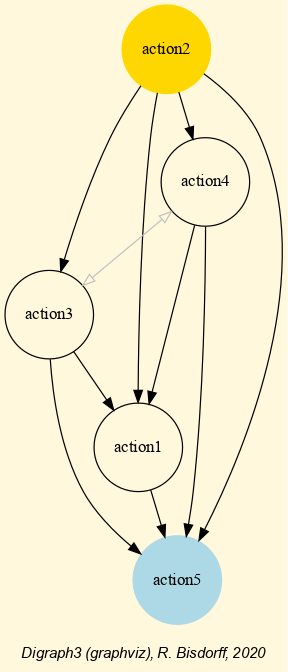
\includegraphics[width=4cm]{Figures/template.png}
\caption{The template outranking digraph models in fact a \textbf{partial order} on the five potential decision alternatives. Alternatives \emph{action3} ($a3$ ) and \emph{action4} ($a4$) appear actually \textbf{incomparable}.}
\label{fig:4.1}       % Give a unique label
\end{figure}

In Listing \ref{list:4.5} their pairwise outranking characteritics show indeed the \textbf{indeterminate} value $0.00$ (Lines 7-8). We may check their pairwise comparison as follows.

\begin{lstlisting}[basicstyle=\footnotesize]
>>> g.showPairwiseComparison('a3','a4')
 *------------  pairwise comparison ----*
  Comparing actions : ('a3','a4')
  crit. wght.  g(x)   g(y)   diff   | ind   pref   r()  | 
   --------------------------------   -----------------
  'g1' 3.00  63.00   23.00  +40.00 | 2.50  5.00  +3.00 | 
  'g2' 3.00   6.00    2.00   +4.00 | 0.00  1.00  +3.00 | 
  'g3' 6.00 -47.30  -35.70  -11.60 | 0.00 10.00  -6.00 | 
  'g4' 2.00  55.40   83.50  -28.10 | 2.09  4.18  -2.00 | 
  'g5' 2.00  63.50   37.50  +26.00 | 0.00 10.00  +2.00 | 
  'g6'  NA   54.90
  Outranking characteristic value:   r(a3 >= a4) = +0.00
  Valuation in range: -18.00 to +18.00
\end{lstlisting}

The incomparability situation between $a3$ and $a4$ results here from a perfect balancing of positive (+8) and negative (-8) criteria significances.

\section{Ranking the template peformance tableau}
\label{sec:4.7}

We may eventually rank the five decision alternatives with a heatmap browser view following the \emph{Copeland} ranking rule (see Section \ref{sec:7.2}) which consistently reproduces the partial outranking order shown in Fig. \ref{fig:4.1}. 

\begin{lstlisting}[basicstyle=\footnotesize] 
   >>> g.showHTMLPerformanceHeatmap(ndigits=1,colorLevels=5,\
   ...    Correlations=True,rankingRule='Copeland',\
   ...    pageTitle='Heatmap of the template performance tableau')
\end{lstlisting}

\begin{figure}[h]
%\sidecaption
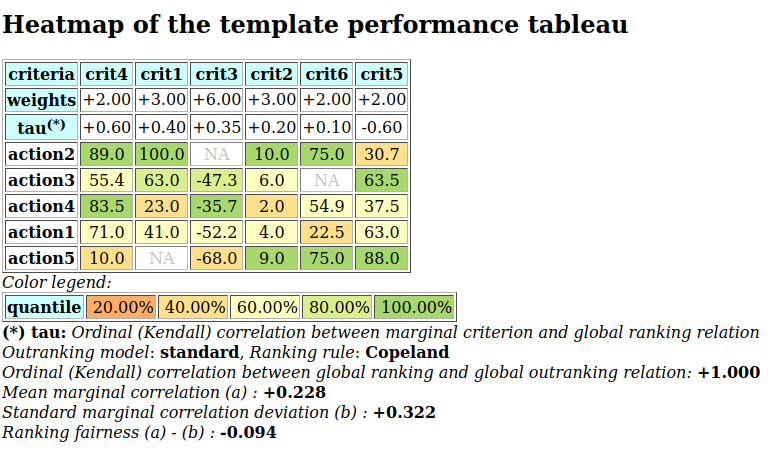
\includegraphics[width=10cm]{Figures/templateHeatmapCop.png}
\caption{Copeland ranked heatmap of the template performance tableau}
\label{fig:4.2}       % Give a unique label
\end{figure}

Due to a 11 against 7 \textbf{plurality tyranny} effect, the \emph{Copeland} ranking rule, essentially based on crisp majority outranking counts, puts here alternative \emph{action5} ($a5$) last, despite its excellent grades observed on criteria $g2$, $g5$ and $g6$. A slightly \textbf{fairer} ranking result may be obtained with the \emph{NetFlows} ranking rule.

\begin{lstlisting}[basicstyle=\footnotesize] 
   >>> g.showHTMLPerformanceHeatmap(ndigits=1,colorLevels=5,\
   ...    Correlations=True,rankingRule='NetFlows',\
   ...    pageTitle='Heatmap of the template performance tableau')
\end{lstlisting}

\begin{figure}[h]
%\sidecaption
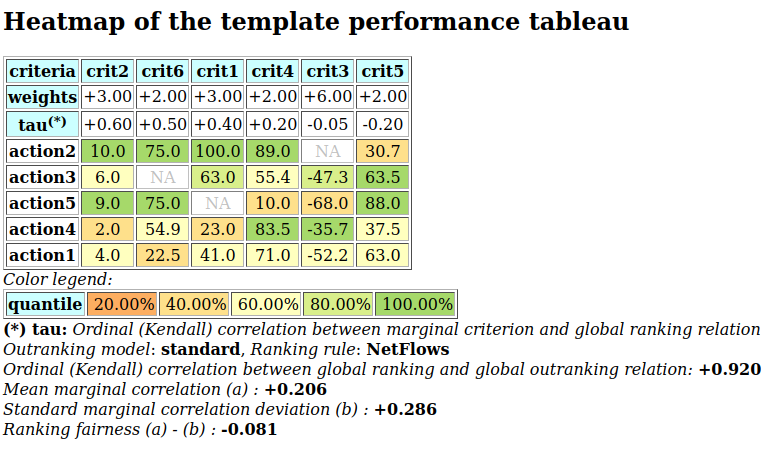
\includegraphics[width=10cm]{Figures/templateHeatmapNF.png}
\caption{Net flows ranked heatmap of the template performance tableau}
\label{fig:4.3}       % Give a unique label
\end{figure}

It might be opportun to furthermore study the robustness of the apparent outranking situations when assuming only *ordinal* or *uncertain* criteria significance weights. If interested in mainly objectively *unopposed* (multipartisan) outranking situations, one might also try the {\tt UnOpposedOutrankingDigraph} constructor. (see Chapter \ref{sec:x}). 
 
